\documentclass{article}

% if you need to pass options to natbib, use, e.g.:
%     \PassOptionsToPackage{numbers, compress}{natbib}
% before loading neurips_2020

% ready for submission
% \usepackage{neurips_2020}

% to compile a preprint version, e.g., for submission to arXiv, add add the
% [preprint] option:
    % \usepackage[preprint,nonatbib]{neurips_2020}

% to compile a camera-ready version, add the [final] option, e.g.:
    \usepackage[final]{neurips_2020}

% to avoid loading the natbib package, add option nonatbib:
    %  \usepackage[nonatbib]{neurips_2020}
\usepackage[british]{babel}
\usepackage{hhline}
\usepackage{bookmark}
\usepackage{multirow}
\usepackage{graphics}
\usepackage{textcomp}
\usepackage{graphicx}
\usepackage{wrapfig}
\usepackage{amsfonts}
\usepackage{algorithm,algorithmicx}
\usepackage{algpseudocode}
\usepackage{microtype}      % microtypography
\usepackage{pdfpages}
\usepackage{amsmath}
\usepackage{amssymb}
\usepackage{float}
\usepackage{amsthm}
\usepackage{multicol}
\usepackage[toc,page]{appendix}
\usepackage{balance} % for balancing columns on the final page
\usepackage{caption} 
\usepackage{hyperref}
\hypersetup{
    colorlinks=true,
    linkcolor=blue,
    urlcolor=blue,
    citecolor=blue
}
\captionsetup[table]{skip=5pt}

\newtheorem{innercustomgeneric}{\customgenericname}
\providecommand{\customgenericname}{}
\newcommand{\newcustomtheorem}[2]{%
  \newenvironment{#1}[1]
  {%
   \renewcommand\customgenericname{#2}%
   \renewcommand\theinnercustomgeneric{##1}%
   \innercustomgeneric
  }
  {\endinnercustomgeneric}
}

\newcustomtheorem{customthm}{Proposition}
\newcustomtheorem{customlemma}{Lemma}

\title{On Variational Generalization Bounds for Unsupervised Visual Recognition}

% The \author macro works with any number of authors. There are two commands
% used to separate the names and addresses of multiple authors: \And and \AND.
%
% Using \And between authors leaves it to LaTeX to determine where to break the
% lines. Using \AND forces a line break at that point. So, if LaTeX puts 3 of 4
% authors names on the first line, and the last on the second line, try using
% \AND instead of \And before the third author name.

\author{
  Karush Suri\\
   University of Toronto\\
  \texttt{karush.suri@mail.utoronto.ca}
}


\begin{document}

\maketitle

\begin{abstract}
Recent advancements in generalization bounds have led to the development of tight information theoretic and data-dependent measures. Although generalization bounds reduce bias in estimates, they often suffer from tractability during empirical evaluation. The lack of a uniform criterion for estimation of Mutual Information (MI) and selection of divergence measures in conventional bounds hinders utility to sparse distributions. To that end, we revisit generalization through the lens of variational bounds. We identify hindrances based on bias, variance and learning dynamics which prevent accurate approximations of data distributions. Our empirical evaluation carried out on large-scale unsupervised visual recognition tasks highlights the necessity for variational bounds as generalization objectives for learning complex data distributions. Approximated estimates demonstrate low variance and improved convergence in comparison to conventional generalization bounds. Lastly, based on observed hindrances, we propose a theoretical alternative which aims to improve learning and tightness of variational generalization bounds. The proposed approach is motivated by contraction theory and yields a lower bound on MI.   
\end{abstract}

\section{Introduction}
Generalization bounds provide tight measures which facilitate the learning of distributions under sparse data. The work of Russo et. al. \cite{russo} has led to drastic improvements \cite{xu,negrea} in bounding generalization error with information theoretic metrics. The surge of information theoretic metrics \cite{xu,bu} has further motivated improvements in bias reduction for control measurements \cite{control}. While generalization bounds tighten the dynamics of sparse learning, a tighter approximation often hurts the performance in the presence of out-of distribution samples \cite{mine}. In many such scenarios, it is difficult to empirically evaluate the performance of the bound \cite{control}. Additionally, the abundance of divergence metrics does not provide a selection criterion for an optimal information theoretic entity \cite{book, measures}. This allows one to rethink the feasibility of conventional bounds in practical scenarios. 

Variational bounds \cite{variational} are a class of probabilistic bounds which depict increasing potential for learning \cite{mine,visual,cpc}. A typical variational bound utilizes a tractable data distribution which can be approximated with limited data samples. This property of variational measures motivates data-efficient learning \cite{cpcv2}. Tractibility of variational bounds for information maximization and minimization allows multiple objective functions to be realisable in a given problem setting \cite{variational}. Variational bounds can then be flexibly modeled as lower and upper bounding measures of information \cite{variational}. However, large-scale utilization of multi-sample variational bounds is an open problem for unsupervised learning tasks \cite{variational}. Data-efficient learning in conjunction with tractable compatibility to data distributions presents variational bounds as suitable candidates for learning objective functions.

We revisit the regime of generalization bounds from the perspective of information theoretic and variational distributions. The work highlights the suitability of variational bounds in comparison to conventional generalization bounds which emphasize only on the bias in data estimates. Variational objectives tackle high bias as well as high variance estimates. Our main contributions are threefold- 

\begin{itemize}
    \item We revisit generalization in light of variational learning and identify hindrances which prevent accurate  approximations of data distributions.
    \item We empirically demonstrate the suitability of variational generalization bounds on unsupervised visual recognition tasks wherein the data distribution is inherently challenging to approximate.  Our evaluation highlights the necessity for variational generalization bounds.
    \item We conjecture a theoretical alternative which aims to address the hindrances discovered in learning variational generalization bounds. The proposed approach is motivated by contraction theory and yields a lower bound on MI. 
  \end{itemize}



\section{Related Work}
\textbf{Variational Bounds}: A number of methods \cite{variational,mine,infomax,cpc,cpcv2} introduce variational bounds for information-based learning. MINE \cite{mine} presents the estimation of MI utilizing gradient descent for high-dimensional random variables. Suitability of MINE leads to improved adversarial generative models and supervised classification tasks. InfoMAX \cite{infomax}, extends the MI framework by simultaneously estimating and maximizing information between output representations and input prior distributions. InfoMAX scales well to unsupervised learning scenarios and sparse latent distributions. While, MINE and InfoMAX highlight the practical utility of information estimation, they do so at the cost of large data requirements from the input distribution. CPC \cite{cpc} and CPCv2 \cite{cpcv2} aid data-efficient learning by introducing the InfoNCE bound. The InfoNCE objective eliminates the need for explicit estimation of MI by providing a lower bound on MI. InfoNCE being a multi-sample bound \cite{variational}, scales well in the number of data samples in-distribution. However, the objective is hindered by large batch sizes and is not tight for large values of MI. The recently proposed interpolation bounds \cite{variational} extend the InfoNCE setup towards a continuum of bounds which trade-off bias with variance. Additionally, the bound is tight for varying batch sizes. Our work is orthogonal to the proposed interpolation scheme and extends it to the generalization setup.  

\textbf{Generalization Bounds}: The pivotal work of \cite{russo} provides a lower-bound on MI based on information-theoretic measures \cite{dv,book}. The MI bound \cite{overfit} is further improved as a result of tight lower bounds on MI minimizing the generalization error \cite{xu,bu}. Additional measures such as data-dependent estimates \cite{negrea} and the specific choice of distributions \cite{kuzborskij} extend the application of lower bounds to stochastic learning dynamics \cite{bu,sgld} and differential privacy \cite{russo}. The bounds are further sharpened using conditional MI \cite{haghifam} in a sample-based framework \cite{steinke} which extends the data-dependent scheme of \cite{negrea}. A more suitable application is the setting of adaptive control \cite{control} which is based on high stochasticity stemming from continuous measurements. The bound provided in \cite{control} aims to address this problem with the introduction of $\alpha$ divergence metrics \cite{measures} which serve as a lower bound on MI. While the bound is proven to be theoretically tight, its application and empirical evaluation remain an open problem in literature. We aim to leverage the theoretical contributions of \cite{control} in order to provide a variational alternative which can be empirically realised.

\textbf{Unsupervised Visual Recognition}: One of the main applications of information-theoretic bounds is unsupervised learning for visual recognition tasks \cite{visual}. The information maximization framework \cite{infomax} reduces local sparsity and motivates the learning of richer representations \cite{cpc}. Multi-sample bounds such as InfoNCE in CPC \cite{cpc} and CPCv2 \cite{cpcv2} contrast augmented representations with actual input samples in order to maximize MI among local pixels. MOCO \cite{moco,mocov2} extends the setup of InfoNCE further with the pretext contrast as a dictionary-lookup task. InfoNCE bound is combined with a momentum encoder which maximizes MI as a slow moving average of input and augmented samples. SimCLR \cite{simclr} builds on the MOCO framework by maximizing the internal agreement between representations. While unsupervised representation learning methods adopt lower bounds on MI, they do so at the cost of large batch sizes. Since the InfoNCE bound is lose at small batch sizes, large architectures lean towards pretraining alternatives \cite{simclrv2} rather than improving lower bounds. The work of \cite{visual} adapts InfoNCE bound based on parameteric and non-parameteric learning of visual instance discrimination. The multi-sample classification is casted to a binary discrimination setup, hence providing improved generalization and consistent performance. Based on this insight, we adopt the instance discrimination setup of \cite{visual} for our experiments. 

\section{Preliminaries}
We review the information-theoretic setup for generalization and variational bounds. Let $X$ and $Y$ be a pair of random variables denoting the input and output data distributions $p(x)$ and $p(y)$ respectively. The mutual information $I(X;Y)$ between $X$ and $Y$ is a reparameterization-invariant measure of dependency consisting of the joint distribution $p(x,y)$and can be mathematically expressed as follows,
\begin{gather}
  I(X;Y) = \mathbb{E}_{p(x,y)}[\log\frac{p(x|y)}{p(x)}] = \mathbb{E}_{p(x,y)}[\log\frac{p(y|x)}{p(y)}] \label{eq:inf}
\end{gather}
\autoref{eq:inf} can be further simplified by expanding the expectation, 
\begin{gather}
  I(X;Y) = \sum_{y}p(x|y)p(y)\log\frac{p(x|y)}{p(x)} = \mathbb{E}_{p(y)}[D_{KL}(p(x|y)||p(x))] \label{eq:infsimp}
\end{gather}
$D_{KL}$ in \autoref{eq:infsimp} denotes the Kullback-Liebler (KL) Divergence \cite{kl} which is a divergence metric. $D_{KL}$ belongs to the general class of $\phi-$divergence metrics $D_{\phi}(P(x)||Q(y))$ which quantify the similarity between any two data distributions $P(x)$ and $Q(y)$. The general form of a $\phi$-divergence, with $\phi$ being a convex and lower semi-continuous function such that $\phi(1)=0$, is expressed in \autoref{eq:phi}. Utilizing $\phi(t)=t\log t$ in \autoref{eq:phi} yields $D_{\phi}(P(x)||Q(y))=D_{KL}(P(x)||Q(y))$.
\begin{gather}
  D_{\phi}(P(x)||Q(y)) = \sum_{y}Q(y)\phi(\frac{P(x)}{Q(y)}) \label{eq:phi}
\end{gather}   
Generalization bounds make use of random variables with a cumulant-generation \cite{cover} function $\psi(\lambda) = \log\mathbb{E}[e^{\lambda x}]$ such that $\lambda \geq 0$. A random variable is called $\sigma$-sub-Gaussian if the argument of the $\log$ cumulant-generation function satisfies $\mathbb{E}[e^{\lambda x}] \leq e^{\frac{\lambda^{2}}{\sigma^{2}}}$ for all $\lambda \in \mathbb{R}$ with $\sigma^{2}$ as the variance proxy or variance factor of the distribution.  
% all background with notations


\section{When Do Bounds Hurt Learning?}
% explain the problems here, demonstrate using table with tick marks and crosses, provide a visual (of distribution) as well, cite examples and mathematical flaws
The work of \cite{variational} throws light on the behavior of tractable distributions with high dimensional random variables. Based on the empirical characteristics of these bounds, one can identify the hindrances faced in generalization of the leanring algorithm (see \autoref{fig:dist}).

\textbf{High Variance}: Normalized upper and lower bounds aid in tractability of variational distributions when the data to be learned is long-tailed. However, these bounds demonstrate high variance as a result of large MI estimates. A suitable alternative to normalized bounds is to adopt the framework of structured bounds. These bounds leverage the structure of the problem and yield a known conditional distribution $p(y|x)$ which is tractable as per the problem setting. Structured bounds are conveniently applicable to representation learning \cite{cpc,variational} but do not necessarily scale to high-dimensional scenarios. Another alternative which provisions a conditional tractable distribution are reparameterization bounds. These bounds make use of an additional functional, known as the \textit{critic}, which converts lower bounds on MI into upper bounds on KL divergence. The critic functional need not explicitly learn the mapping between $x$ and $y$. However, reparameterization is only made feasible if the conditional distribution $p(y|x)$ is tractable. 

\textbf{High Bias}: Unnormalized upper and lower bounds demonstrate high bias and hurt tractability of complex distributions. Primary reasons for instability in bounds is lack of a partition functional which normalizes MI estimates. \cite{variational} argues that requirement of a partition function presents high bias as a result of exponential distributions which may not be tractable. However, the work does not provide empirical evidence on their tractability which leaves the suitability of a normalization constant an open question. A suitable alternative to address biased estimates is the adoption of density ratios which train the critic functional using a divergence metric. The Jensen-Shanon Divergence (JSD) is one such scheme which yields a lower-biased estimate of optimal critic. While training critics is theoretically suitable, empirical evaluations \cite{variational} demonstrate unstable convergence of exponential gradients. 

\begin{figure*}[ht]
  \centering
  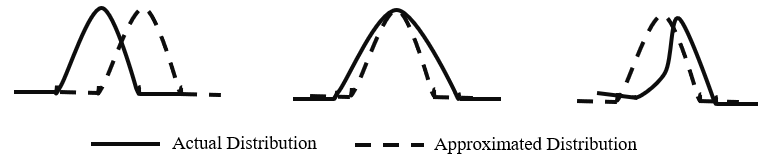
\includegraphics[height=2.75cm,width=13cm]{dist.PNG}
  \caption{\textbf{Left} Conventional lose bounds suffer from high bias which hurts generalization of the learnt distribution, \textbf{Center} Learnt distribution is additionally hampered with noisy approximations, \textbf{Right} Biased estimates in conjunction with noisy dynamics hurt the completeness of learnt distribution.}
  \label{fig:dist}
\end{figure*}

\textbf{A Failure to Learn}: Biased and noisy estimates are the key hindrances in learning tractable distributions. To that end, \cite{variational} aptly proposes a continuum of multi-sample interpolation bounds which trade-off bias with variance. A simpler form of critic when applied to non-linear interpolation in InfoNCE samples yields a continuum of lower bounds on MI. The new bound can be manually tuned using $\gamma$ which trades off bias with variance. Nonlinear interpolation bounds proposed in conjunction with MI saturate at $\log \frac{K}{\gamma}$ with $K$ being the number of samples in the batch. Saturation of interpolation hurts the completeness of distribution and the bound fails to learn large MI estimates with increasing batch sizes.  

% demonstrate DV empirically and highlight its consequences
% highlight the importance of alpha I and difficulty in selection of optimal alpha

\section{Variational Bounds for Generalization}
This section provides insights into variational bounds as generelization measures of MI. Learning of variational bounds is discussed from the multi-sample and interpolation perspective. Nonlinear interpolation bounds give rise to the trade-off between bias and variance in estimates. Following generalization through this lens, we formulate an alternate approach with bias reduction as a contraction mapping. We extend our theoretical claims to previously discussed generalization bounds and discuss their formulations.
% explain what the section is about and what you wish to accomplish, make sure to be mathematical

\subsection{Learning Variational Bounds}
% review the bounds here, critically comment on their usage
\textbf{InfoNCE}: The InfoNCE objective is based on multi-sample unnormalized bounds. These bounds formulate multi-sample MI $I(X_{1};Y)$ which is bounded by the optimal choice of critic $f(x,y)$. One such formulation is based on MINE \cite{mine} as presented in \autoref{eq:mine}.
\begin{gather}
  I(X_{1},Y) \geq 1 + \mathbb{E}_{p(x_{1:K})p(y|x_{1})}[\log\frac{e^{f(x_{1},y)}}{m(y;x_{1:K})}] - \mathbb{E}_{p(x_{1:K})p(y)}[\log\frac{e^{f(x_{1},y)}}{m(y;x_{1:K})}] \label{eq:mine}
\end{gather} 
Here $m(y;x_{1:K})$ is a Monte-Carlo estimate of the partition function $Z(y)$ and is mathematically expressed in \autoref{eq:monte}.
\begin{gather}
  m(y;x_{1:K}) = \frac{1}{K}\sum_{k=1}^{K}e^{f(x_{k},y)} \label{eq:monte}
\end{gather}
One can recover the InfoNCE bound ($I_{NCE}$) upon averaging over all $K$ replicates in the last term of \autoref{eq:mine} which yields 1. $I_{NCE}$ can then be expressed as a lower bound on MI in \autoref{eq:nce}.
\begin{gather}
  I(X;Y) \geq \mathbb{E}[\frac{1}{K}\sum_{k=1}^{K}\log\frac{e^{f(x_{k},y_{k})}}{\frac{1}{K}\sum_{j=1}^{K}e^{f(x_{k},y_{j})}}] \triangleq I_{NCE} \label{eq:nce}
\end{gather} 

\textbf{Nonlinear Interpolation}: The multi-sample framework of MINE can be further extended using a simpler formulation. A nonlinear interpolation between MINE and $I_{NCE}$ bridges the gap between low-bias and high-variance estimates of MINE with high-bias and low-variance estimates of $I_{NCE}$. The nonlinear interpolation bound ($I_{IN}$) is expressed in \autoref{eq:non}.
\begin{multline}  
  I_{IN} \triangleq 1 + \mathbb{E}_{p(x_{1:K})p(y|x_{1})}[\log\frac{e^{f(x_{1},y)}}{\gamma m(y;x_{1:K})+(1-\gamma)q(y)}]\\ - \mathbb{E}_{p(x_{1:K})p(y)}[\log\frac{e^{f(x_{1},y)}}{\gamma m(y;x_{1:K})+(1-\gamma)q(y)}] \label{eq:non}
\end{multline}  
While $I_{NCE}$ is upper bounded by $\log K$, $I_{IN}$ is upper bounded by $\log \frac{K}{\gamma}$. The control in bias-variance trade-off improves accuracy of estimates. However, the significance of $\gamma$ remains an open question in the case of higher-order divergence metrics and large value of MI in practical settings. 

\textbf{$\phi$-divergence}: Generalized divergence metrics facilitate tighter bounds by utilizing $\alpha$-MI as the dependence measure. \cite{control} presents a tight bound which is based on random variables with cumulant-generation functions. If $X_{i}-Y_{i}$ has a cumulant generation function $\leq \psi_{i}(\lambda)$ over domain $[0,b_{i})$ where $0 \leq b_{i} \leq \infty$ and $\psi_{i}(\lambda)$ is convex and $i$ denotes the iterates of the variables $X$ and $Y$, one can define the expected cumulant-generation function $\bar{\psi_{i}}(\lambda)$ as in \autoref{eq:expcum} to obtain the bound expressed in \autoref{eq:bound}. Here, $\bar{\psi}^{*-1}$ denotes the inverse of the convex conjugate of $\bar{\psi}$. 
\begin{gather}
  \bar{\psi}(\lambda) = \mathbb{E}_{i}[\psi_{i}(\lambda)],\; \lambda \in [0,\underset{i}{\min} b_{i}) \label{eq:expcum}
\end{gather}
\begin{gather}
  \mathbb{E}[X_{i} - Y_{i}] \leq \bar{\psi}^{*-1}(I(X;Y)) \label{eq:bound}
\end{gather} 
The bound of \cite{control} generalizes the work of \cite{russo} as it is applicable to long-tailed distributions and variables which may not necessarily obey the sub-Gaussianity assumption. Based on \autoref{eq:bound}, \cite{control} formulates the $\alpha$-MI bound which improves the bound presented in \cite{russo}. Suppose $||X_{i} - Y_{i}||_{\beta} \leq \sigma_{i}$ where $1 \leq \beta \leq \infty$, if $\alpha \triangleq$ conjugate of $\beta$ such that $\frac{1}{\alpha} + \frac{1}{\beta} = 1$, then the improved $\alpha$-MI bound can be expressed as in \autoref{eq:impbound}. 
\begin{gather}
  |\mathbb{E}[X_{i} - Y_{i}]| \leq ||\sigma||_{\beta}I_{\alpha}(X;Y)^{\alpha} \label{eq:impbound}
\end{gather}
While the bound in \autoref{eq:impbound} is generalizable to variables with no moment-generating functions, its tightness remains an open question. \cite{control} prove the tightness of \autoref{eq:impbound} using extreme value theory. The bound is tight for $n^{\frac{1}{\beta}}$ with $n$ being the number of data samples. However, tightness holds under the condition that $\beta$ is bounded such that $2 \leq \beta \leq \infty$. For large values of $\beta$, $n^{\frac{1}{\beta}}$ tends to diminish which renders the estimation of $I_{\alpha}(X;Y)$ intractable. Moreover, $\phi$-divergences are originally defined as power functions over $\beta$ while the bound makes use of an affine transformation. The alternate formulation may not hold in the more generalized-case. This poses a hindrance for $\alpha$-MI bounds to be used as substitutes to pre-existing methods. 

\subsection{Improving Bounds on MI}
% provide your novelty, explain its usage well
% maybe use extreme value theory to prove the tightness of InfoNCE
% maybe combine InfoNCE with control bound
The bound expressed in \autoref{eq:bound} can be improved by using the multi-sample InfoNCE bound. This arises as a direct consequence of the fact that $I(X;Y) \geq I_{NCE}$. We formalize this finding in Proposition \autoref{one} and defer all proofs to Appendix. 
\begin{customthm}{1}\label{one}
  If $X_{i}-Y_{i}$ has the expected cumulant-generation function $\bar{\psi_{i}}(\lambda)$ and the inverse of the convex conjugate of $\bar{\psi}$ denoted by $\bar{\psi}^{*-1}$ exists, then the improved bound utilizing $I_{NCE}$ can be expressed as follows,
\begin{gather}
  \mathbb{E}[X_{i} - Y_{i}] \leq \bar{\psi}^{*-1}(I_{NCE}) \label{eq:newbound}
\end{gather} 
\end{customthm}
While Proposition \autoref{one} presents an improvement over the original bound, the expression makes use of $I_{NCE}$ which demonstrates high bias and saturation at $\log K$. This motivates the need for a bound which can retain the tightness of $I_{NCE}$ and at the same time trade off bias with variance. 

To address the improvement of generlization bound, we turn our attention to non-linear interpolation bound $I_{IN}$ introduced in the previous section. Interpolation aids in the trade off between bias and variance and improves the bound's stability at larger batch sizes. More specifically, $I_{IN}$ saturates at $\log \frac{K}{\gamma}$. However, the tightness of $I_{IN}$ with respect to $I_{NCE}$ cannot be validated as a result of nonlinear iterates during interpolation. For $\gamma\neq 1$, $I_{IN} \neq I_{NCE}$ which poses a hindrance in the comparison of $I_{IN}$ to $I_{NCE}$. However, a lower bound on $I_{IN}$ can yield a lower bound on $I_{NCE}$ with high probability since $I_{IN} = I_{NCE}$ at $\gamma=1$. Thus, obtaining a tractable lower bound on $I_{IN}$ would further improve generlization and strengthen the claim of Proposition \autoref{one}. 

One can leverage contraction theory \cite{banach, contraction} to highlight mathematical properties which would aid in extracting a tractable bound. Such a mapping guarantees convergence in asymptotically-stable nonlinear systems \cite{contraction} and provides a dynamical framework for assessing stability of bounds \cite{sql}. A contraction mapping between any two functions $f_{1}(w)$ and $f_{2}(w)$ implies that the norm distance between $f_{1}(w)$ and $f_{2}(w)$ decays at a constant (in some cases geometric \cite{banach}) rate. Given a contraction operator $\tau$ when iteratively applied on $f_{1}(w)$ and $f_{2}(w)$, the mapping $\tau f_{1}(w) - \tau f_{2}(w)$ is a contraction if the inequality in \autoref{eq:contraction} is satisfied.
\begin{gather}
  \tau f_{1}(w) - \tau f_{2}(w) \leq ||f_{1}(w) - f_{2}(w)||,\; \forall w \label{eq:contraction}
\end{gather} 
\autoref{eq:contraction} is a generalization of the fixed-point theory in Banach metric spaces \cite{contraction} which provides suitable conditions for assessing stability of nonlinear systems. The key component of evaluating a nonlinear system is motivated by its convergence towards a fixed point in the Banach metric space. Convergence towards a fixed point indicates stability of the overall mapping. We borrow from this insight in order to form a contraction on nonlinear interpolation bounds which can be interpreted as a continuum in a nonlinear space. Upon realizing input samples as points in this continuous nonlinear space, a simple yet elegant formulation of a contraction mapping can be achieved. To utilize a contraction mapping on $I_{IN}$, we seek a contraction operator $\mathcal{T}$ which is tractable. A suitable choice is the alternate Boltzmann (mellowmax) operator introduced in \cite{mellowmax}. The Mellowmax operator $\mathcal{T}f(w)=\log \sum_{w} \exp{f(w)}$ which may be interpreted as an energy-based function. Retaining properties of the Boltzmann distribution, mellowmax is an asymptotically stable formulation of the Gibbs distribution. Mellowmax has been suitably adopted in control and learning settings \cite{sql,emix} wherein the probability distribution forms a continuum over the input space. Additionally, the exponent in $\mathcal{T}$ is tractable as it is followed by the $\log$ which prevents the arguments from exploding. Proposition \autoref{two} depicts the contraction property of $\mathcal{T}$. 
\begin{customthm}{2}\label{two}
  Given a function $f(w):w\rightarrow \mathbb{R}$, the operator $\mathcal{T}f(w)=\log \sum_{w} \exp{f(w)}$ forms a contraction on $f(w)$. 
\end{customthm}
We leverage the result of Proposition \autoref{two} to obtain a tractable lower bound on $I_{IN}$. This requires summing over interpolating samples $1:K$ of the distribution. The novel bound $I_{N}$ obtained by operating $\mathcal{T}$ on interpolation terms is expressed in Proposition \autoref{prop3}. Note that the sum in the first interpolation term requires computation of the inner expectation which now depends on the distribution conditioned on each iterate. This facilitates tractability since the estimates obtained as a result of individual conditioning would be accurate in comparison to estimates based on a single sample. 
\begin{customthm}{3}\label{prop3}
  If the operator $\mathcal{T}f(w)=\log \sum_{w} \exp{f(w)}$ is a contraction mapping $\forall w$, then the nonlinear interpolation bound $I_{IN}$ can be further simplified as expressed in \autoref{eq:novelbound}. 
\begin{multline}  
  I_{IN} \geq I_{N} \triangleq 1 + \log \sum_{i=1}^{K} \exp{\mathbb{E}_{p(x_{1:K})p(y|x_{i})}[\log\frac{e^{f(x_{i},y)}}{\gamma m(y;x_{1:K})+(1-\gamma)q(y)}]}\\ + \log \sum_{i=1}^{K} \exp{\mathbb{E}_{p(x_{1:K})p(y)}[\log\frac{e^{f(x_{i},y)}}{\gamma m(y;x_{1:K})+(1-\gamma)q(y)}]} \label{eq:novelbound}
\end{multline} 
\label{novelbound} 
\end{customthm}
\autoref{eq:novelbound} is a lower bound on $I_{IN}$ which indicates that the novel bound $I_{N}$ is also a lower bound on $I_{NCE}$ with high probability since $I_{IN} = I_{NCE}$ at $\gamma=1$. Thus, one can safely make the following claim,
\begin{gather}
  I(X;Y) \geq I_{NCE} \geq I_{N} \label{eq:main}
\end{gather}
\autoref{eq:main} can be further used to validate the suitability of the novel bound $I_{N}$ as a replacement to $I_{NCE}$ in Proposition \autoref{one}. This leads us to formulate the new generalization bound.
\begin{customthm}{4}\label{prop4}
  Since $I_{NCE} \geq I_{N}$ with high probability, the generalization bound in Proposition \autoref{one} can be simplified as follows,
  \begin{gather}
    \mathbb{E}[X_{i} - Y_{i}] \leq \bar{\psi}^{*-1}(I_{N}) \leq \bar{\psi}^{*-1}(I_{NCE})
  \end{gather} 
\end{customthm}
Proposition \autoref{prop3} and Proposition \autoref{prop4} obtained as a result of \autoref{eq:contraction} highlight the main findings of our work. Theoretically, $I_{N}$ retains the properties of $I_{IN}$ and would depict convergence analogous to $I_{IN}$ in settings with large batch sizes. Additionally, the bias-variance trade off arising as a virtue of nonlinear interpolation presents $I_{N}$ as a suitable replacement to $I_{NCE}$ in Proposition \autoref{one}. On the other hand, an empirical comparison of stability between $I_{NCE}$ and $I_{N}$ may be difficult to observe. This arises as a direct consequence of interpolation combined with dimensional contraction which may lead $I_{N}$ to collapse for some iterates. Although theoretical in nature, our findings motivate empirical validation and application of the proposed bound. 
\section{Experiments}
% state your objectives and what you wish to assess
Our experiments aim to evaluate the suitability of variational bounds in the generalization setup. More specfically, we aim to answer the following two questions; (1) Which variational bounds are suitable for generalization settings? and (2) How do these bounds scale to large number of samples in data distribution? 

\subsection{Setup}
Our experiments consist of unsupervised instance discrimination tasks \cite{visual} which involve the recognition of images based on MI. The setup consists of three standard benchmarks; MNIST, FashionMNIST and CIFAR10, and two large-scale datasets; EMNIST (Letters) and CIFAR100. In order to study the effect of deep architectures we employ ResNET-18 and ResNet-34 modules. The comparison consists of 4 different MI objectives with InfoNCE (as expressed in $I_{NCE}$) and Donsker-Vardhan (DV) loss (based on \cite{infomax}) as conventional objectives and Jensen-Shannon Divergence (JSD) and Reverse KL (RKL) as $\phi$-divergence measures. Each objective maximizes similarity between logits and feature representations. The fully-supervised Cross-Entropy (CE) is additionally considered as a baseline. Objectives on the standard benchmarks are trained and evaluated for 200 epochs while large-scale datasets make use of 600 epochs. We direct the curious reader to Appendix for experiment details and hyperparameters.  
% explain the setup 

\subsection{Unsupervised Instance Discrimination}
% provide tabular results, emphasize on whay and how

\begin{table*}[ht]
  \centering
  \renewcommand{\arraystretch}{1.2}
  \resizebox{\textwidth}{!}{
  \begin{tabular}{c|c|c|c|c|c|c|c|c|c|c|c}
    Architecture & Datasets & \multicolumn{2}{c|}{CE} & \multicolumn{2}{c|}{JSD} & \multicolumn{2}{c|}{DV} & \multicolumn{2}{c|}{InfoNCE} & \multicolumn{2}{c}{RKL}\\
    % \hline
    % \textbf{Inactive Modes} & \textbf{Description}\\
    \cline{3-12}
    & & Gen. Error & Top1 Acc. & Gen. Error & Top1 Acc. & Gen. Error & Top1 Acc. & Gen. Error & Top1 Acc. & Gen. Error & Top1 Acc.\\
    %\hhline{~--}
    \hline
     & MNIST & 0.02 & 95.55 & 0.08 & 92.04 & 6.27 & 32.16 & 0.13 & \textbf{92.34} & \textbf{0.06} & 90.86\\
     & FashionMNIST & 0.11 & 95.13 & \textbf{0.06} & \textbf{92.41} & 3.64 & 29.44 & 0.11 & 92.24 & \textbf{0.06} & 92.25\\
    ResNet-18 & EMNIST & 0.15 & 81.02 & 0.04 & 80.40 & - & 31.57 & 0.07 & \textbf{81.13} & \textbf{0.03} & 80.65\\
     & CIFAR10 & 0.10 & 80.57 & \textbf{0.04} & 71.18 & 1.17 & 31.29 & 0.07 & 70.09 & 0.05 & \text{71.36}\\
     & CIFAR100 & 0.17 & 52.02 & \textbf{0.05} & 40.59 & 1.67 & 10.06 & 0.13 & \textbf{41.24} & 0.08 & 39.28\\ \hline
     & MNIST & 0.12 & 96.59 & 0.05 & 92.82 & 2.85 & 24.40 & \textbf{0.04} & \textbf{93.10} & 0.06 & 92.97\\
     & FashionMNIST & 0.09 & 96.37 & \textbf{0.04} & 93.32 & 9.10 & 28.96 & 0.13 & 93.08 & 0.08 & \textbf{93.47}\\
    ResNet-34 & EMNIST & 0.09 & 83.43 & \textbf{0.03} & 80.66 & - & 16.97 & 0.07 & \textbf{83.16} & 0.04 & 83.10\\
     & CIFAR10 & 0.13 & 81.81 & \textbf{0.04} & 71.65 & 1.23 & 27.24 & 0.08 & 71.87 & 0.06 & \textbf{72.42}\\
     & CIFAR100 & 0.13 & 52.45 & 0.08 & 37.92 & 1.89 & 7.41 & 0.15 & 39.75 & \textbf{0.07} & \textbf{42.04}\\ \hline
  \end{tabular}}
  \caption{Summary of results based on Generalization Error (Gen. Error) and Top1 Accuracy (Acc) for all objectives on standard and large-scale benchmarks using ResNet-18 and ResNet-34 models. Highlighted entries depict best performing objectives in the unsupervised setting. $\phi$-divergence measures such as JSD and RKL depict improved generalization and performance comparable to conventional MI-based InfoNCE and fully-supervised CE. The DV objective on the other hand, demonstrates instability as a result of exponential estimates. For complete results on bias and variance refer to Appendix.}
  \label{tab:table}
\end{table*}
\begin{figure*}[ht]
\centering
  
\includegraphics[height=2.5cm,width=14cm]{18_gen_error.png}
  \caption{Gen. Error for variational objectives on standard and large-scale benchmarks for the ResNet-18 model. $\phi$-divergence measures demonstrate improved stability and generalization in comparison to conventional InfoNCE and fully-supervised CE which depict high bias. Conventional DV, on the other hand, presents high variance and unstable convergence as a result of exponential estimates of the partition function.}
  \label{fig:plot}
\end{figure*}
\autoref{tab:table} presents the summary of results obtained from our empirical study of objectives. We compare generalization and performance of objectives based on Generalization Error (Gen. Error) and Top1 Classification Accuracy (Acc.) on standard and large-scale benchmarks using ResNet-18 and ResNet-34 models. Empirical evaluation of objectives depicts improved generalization of $\phi$-divergence based objectives in comparison to conventional InfoNCE and the fully-supervised setting of CE. JSD is found to be stable and best minimizes the generalization error on 6 out of the 10 scenarios. RKL, on the other hand, yields competitive generalization and stability in comparison to JSD. InfoNCE demonstrates high bias among MI-based objectives. This is found to be consistent with the claims of \cite{variational} which highlight the necessity for accurate multi-sample objectives. DV objective depicts instability in convergence arising from high bias and variance in its estimates. The claims of \cite{variational} and \cite{infomax} support this empirical result. Large values of exponential estimates in conjunction with the requirement of a partition function pose hindrance to generalization. This hampers the utility of DV as an unsupervised learning objective. 

One can compare the suitability of variational objectives across different architectures in order to best evaluate performance. JSD depicts consistent performance across ResNet-18 and ResNet-34 architectures. Additionally, JSD scales well to large-scale datasets and maintains a minimum generalization error. RKL, on the other hand, demonstrates suitability for ResNet-18 but falls short of optimum generalization on the deeper ResNet-34 model. Surprisingly, RKL depicts accurate recognition performance at test time which is indicative of its potential as an unsupervised objective. While JSD and RKL generalize well, they present high bias in their estimates. This is indicative of a moderately accurate performance at execution time. InfoNCE, on the other hand, depicts low variance in its estimates which results in the most accurate performance in the unsupervised setting. Additionally, the performance of InfoNCE is matched for shallow as well as deeper architectures. However, saturation of $I_{NCE}$ at large batch sizes and samples leads to a lose bound. This is indicative of its performance on large-scale datasets which consist of a larger number of negative samples and classes. The claim is further strengthened in \cite{variational} wherein MI estimates may take large values and lead to sub-optimal convrgence. 

To better understand convergence and tightness of variational bounds, once can gain visual insights into their behavior during learning. \autoref{fig:plot} presents comparison of generalization error during training for all objectives on standard and large-scale benchmarks utilizing the ResNet-18 architecture. Insights obtained from \autoref{fig:plot} validate our claims on generalization drawn from \autoref{tab:table}. Unsupervised variational objectives demonstrate improved generalization as a result of minimimum validation error in comparison to the fully-supervised CE objective. Moreover, consistency of these objectives across all datasets validates stability in convergence. Out of unsupervised objectives, JSD and RKL demonstrate equivalent errors with JSD slightly outperforming the latter. Suitability of JSD on standard and large-scale datasets further validates its robustness to large sample sizes. This is not found consistent in InfoNCE which depicts slightly higher errors and delayed convergence on EMNIST and CIFAR100 datasets. Furthermore, instability of DV bound is validated as a result of no loss signal in the gradient. We direct the reader to Appendix for complete results.  

\section{Discussion}
Generalization bounds present significant promise for yielding accurate learning algorithms. However, these bounds are often held intractable during empirical evaluation. To this end, we have revisited the generalization setup from the perspective of variational bounds of MI. Firstly, we identified failure modes which hinder a bound to learn data as a result of bias and variance in estimates. Based on these estimates, we formulate a theoretical alternative which is based on contraction theory and nonlinear interpolation bounds. The novel $I_{N}$ bound is a lower bound on nonlinear interpolation bound $I_{IN}$, and hence the InfoNCE bound $I_{NCE}$ with high probability. We then carry out empirical evaluations of variational bounds under the generalization setup in order to identify potential generalization candidates. Our study highlights the suitability of $\phi$-divergences in $\alpha$-MI as suitable alternatives for generalization. Specifically, JSD and RKL demonstrate improved generalization on datasets with small and large sample sizes. Their performance is additionally found consistent on deeper architectures. 

While our study establishes a suitable link between generalization and variational bounds, it presents three main shortcomings. Firstly, tightness and validity of our novel $I_{N}$ bound is demonstrated theoretically. In the near future we would like to empirically evaluate the suitability of the bound and its corresponding claims. Secondly, our empirical evaluation consists of datasets with well-suited classes. A more thorough approach of evaluating generalization bounds could include unbalanced and larger number of classes as found in the ImageNet benchmark. Lastly, evaluation of bounds on a more diverse set of architectures would yield insights towards their stability and failure modes. We leave these for our future work.  

\bibliographystyle{unsrt} 
\small{\bibliography{sample}}

\newpage
\appendix
\section{Proofs}
\begin{customthm}{1}
  If $X_{i}-Y_{i}$ has the expected cumulant-generation function $\bar{\psi_{i}}(\lambda)$ and the inverse of the convex conjugate of $\bar{\psi}$ denoted by $\bar{\psi}^{*-1}$ exists, then the improved bound utilizing $I_{NCE}$ can be expressed as follows,
\begin{gather}
  \mathbb{E}[X_{i} - Y_{i}] \leq \bar{\psi}^{*-1}(I_{NCE}) \nonumber
\end{gather} 
\end{customthm}
\begin{proof}
  The proof is straightforward and based on original generalization bound in \autoref{control}. The result is obtained by following the steps of Theorem 2 \cite{control} and replacing $I(X_{i};Y_{i})$ with $I_{NCE}$ in the last step as follows,
  \begin{gather}
    \mathbb{E}[X_{i} - Y_{i}] \leq \underset{\lambda \in [0,\min_{i}b_{i})}{\inf} \frac{\bar{\psi}(\lambda)+I(X_{i};Y_{i})}{\lambda} \nonumber \\
    \mathbb{E}[X_{i} - Y_{i}] \leq \underset{\lambda \in [0,\min_{i}b_{i})}{\inf} \frac{\bar{\psi}(\lambda)+I_{NCE}}{\lambda}; \;\text\;{since} I_{NCE} \leq I(X_{i};Y_{i}) \nonumber\\
    = \bar{\psi}^{*-1}(I_{NCE}) \nonumber
  \end{gather}
  This completes the proof.
\end{proof}

\begin{customthm}{2}
  Given a function $f(w):w\rightarrow \mathbb{R}$, the operator $\mathcal{T}f(w)=\log \sum_{w} \exp{f(w)}$ forms a contraction on $f(w)$. 
\end{customthm}
\begin{proof}
  Let us first define a norm on the functions $||f_{1}(w) - f_{2}(w)|| \equiv \underset{w}{max}|f_{1}(w) - f_{2}(w)|$. Suppose $\epsilon = ||f_{1}(w) - f_{2}(w)||$,
  \begin{gather}
      \log \sum_{w}\exp{(f_{1}(w))} \leq \log \sum_{w}\exp{(f_{2}(w) + \epsilon)} \nonumber \\
      = \log \sum_{w}\exp{(f_{1}(w))} \leq \log \exp{(\epsilon)} \sum_{w}\exp{(f_{2}(w))} \nonumber \\
      = \log \sum_{w=1}\exp{(f_{1}(w))} \leq \epsilon + \log \sum_{w} \exp{(f_{2}(w))} \nonumber \\
      = \log \sum_{w} \exp{(f_{1}(w))} - \log \sum_{w} \exp{(f_{2}(w))} \leq ||f_{1}(w) - f_{2}(w)|| \label{eq:case1}
  \end{gather}
  Similarly, using $\epsilon$ with $\log \sum_{w} \exp{(f_{1}(w))}$,
  \begin{gather}
      \log \sum_{w}\exp{(f_{1}(w) + \epsilon)} \geq \log \sum_{w}\exp{(f_{2}(w))} \nonumber \\
      = \log \exp{(\epsilon)}\sum_{w}\exp{(f_{1}(w))} \geq \log \sum_{w}\exp{(f_{2}(w))} \nonumber \\
      = \epsilon + \log \sum_{w} \exp{(f_{1}(w))} \geq \log \sum_{w}\exp{(f_{2}(w))} \nonumber \\
      = ||f_{1}(w) - f_{2}(w)|| \geq \log \sum_{w} \exp{(f_{2}(w))} - \log \sum_{w} \exp{(f_{1}(w))} \label{eq:case2}
  \end{gather}
  Results in \autoref{eq:case1} and \autoref{eq:case2} prove that $\mathcal{T}$ is a contraction. 
\end{proof}

\begin{customthm}{3}
  If the operator $\mathcal{T}f(w)=\log \sum_{w} \exp{f(w)}$ is a contraction mapping $\forall w$, then the nonlinear interpolation bound $I_{IN}$ can be further simplified as expressed in \autoref{eq:novelbound}. 
\begin{multline}  
  I_{IN} \geq I_{N} \triangleq 1 + \log \sum_{i=1}^{K} \exp{\mathbb{E}_{p(x_{1:K})p(y|x_{i})}[\log\frac{e^{f(x_{i},y)}}{\gamma m(y;x_{1:K})+(1-\gamma)q(y)}]}\\ \log \sum_{i=1}^{K} \exp{\mathbb{E}_{p(x_{1:K})p(y)}[\log\frac{e^{f(x_{i},y)}}{\gamma m(y;x_{1:K})+(1-\gamma)q(y)}]} \nonumber
\end{multline} 
\end{customthm}
\begin{proof}
  From \autoref{eq:non}, we have the following,
  \begin{multline}  
    I_{IN} \triangleq 1 + \mathbb{E}_{p(x_{1:K})p(y|x_{1})}[\log\frac{e^{f(x_{1},y)}}{\gamma m(y;x_{1:K})+(1-\gamma)q(y)}]\\ - \mathbb{E}_{p(x_{1:K})p(y)}[\log\frac{e^{f(x_{1},y)}}{\gamma m(y;x_{1:K})+(1-\gamma)q(y)}] \nonumber
  \end{multline}  
For notational convenience, we relabel the two interpolation terms as follows,
\begin{gather*}
  \mathcal{P}(x) = \mathbb{E}_{p(x_{1:K})p(y|x_{1})}[\log\frac{e^{f(x_{1},y)}}{\gamma m(y;x_{1:K})+(1-\gamma)q(y)}]\\ \mathcal{Q}(x) = \mathbb{E}_{p(x_{1:K})p(y)}[\log\frac{e^{f(x_{1},y)}}{\gamma m(y;x_{1:K})+(1-\gamma)q(y)}]
\end{gather*}
Using the result from Proposition \autoref{two} and applying $\mathcal{T}$ to the two interpolation terms in the expressions gives us the following,
\begin{gather*}
  \mathcal{T}\mathcal{P}(x) - \mathcal{T}\mathcal{Q}(x) \leq \underset{x}{max}|\mathcal{P}(x) - \mathcal{Q}(x)| \\
  \mathcal{T}\mathcal{P}(x) - \mathcal{T}\mathcal{Q}(x) \leq \mathcal{P}(x) - \mathcal{Q}(x)
\end{gather*}  
Using the above result in $I_{IN}$ yields the lower bound $I_{N}$ and completes the proof.
\end{proof}  

\begin{customthm}{4}
  Since $I_{NCE} \geq I_{N}$ with high probability, the generalization bound in Proposition \autoref{one} can be simplified as follows,
  \begin{gather}
    \mathbb{E}[X_{i} - Y_{i}] \leq \bar{\psi}^{*-1}(I_{N}) \leq \bar{\psi}^{*-1}(I_{NCE}) \nonumber
  \end{gather} 
\end{customthm}
\begin{proof}
  We follow the steps of Proposition \autoref{one} to obtain the lower bound with $I_{NCE}$ and replace it with $I_{N}$ as follows,
  \begin{gather}
    \mathbb{E}[X_{i} - Y_{i}] \leq \underset{\lambda \in [0,\min_{i}b_{i})}{\inf} \frac{\bar{\psi}(\lambda)+I(X_{i};Y_{i})}{\lambda} \nonumber \\
    \mathbb{E}[X_{i} - Y_{i}] \leq \underset{\lambda \in [0,\min_{i}b_{i})}{\inf} \frac{\bar{\psi}(\lambda)+I_{NCE}}{\lambda}; \;\text\;{since} I_{NCE} \leq I(X_{i};Y_{i}) \nonumber\\
    \mathbb{E}[X_{i} - Y_{i}] \leq \underset{\lambda \in [0,\min_{i}b_{i})}{\inf} \frac{\bar{\psi}(\lambda)+I_{N}}{\lambda}; \;\text\;{since} I_{N} \leq I_{NCE} \nonumber\\
    = \bar{\psi}^{*-1}(I_{N}) \nonumber
  \end{gather}
  This completes the proof.

\end{proof}

\section{Additional Results}
\subsection{ResNet-18}
\begin{figure}[H]
  \centering
    
\includegraphics[height=2.5cm,width=14cm]{18_gen_error.png}
    \caption{Gen. Error for variational objectives on standard and large-scale benchmarks for the ResNet-18 model. $\phi$-divergence measures demonstrate improved stability and generalization in comparison to conventional InfoNCE and fully-supervised CE which depict high bias. Conventional DV, on the other hand, presents high variance and unstable convergence as a result of exponential estimates of the partition function.}
  \end{figure}
  \begin{figure}[H]
    \centering
      
\includegraphics[height=2.5cm,width=14cm]{18_top1_acc.png}
      \caption{Comparison of Top1 classification accuracies for variational objectives on standard and large-scale benchmarks for the ResNet-18 model. While fully-supervised CE demonstrates best performance, InfoNCE and $\phi$-divergence measures depict comparably accurate performance. Conventional DV, on the other hand, demonstrates a failure to learn.}
    \end{figure}
    \begin{figure}[H]
      \centering
        
\includegraphics[height=2.5cm,width=14cm]{18_top5_acc.png}
        \caption{Comparison of Top5 classification accuracies for variational objectives on standard and large-scale benchmarks for the ResNet-18 model. Performance is analogous to Top1 counterpart with variational bounds demonstrating improved performance on standard mnist and fashionmnist benchmarks.}
      \end{figure}
      
\subsection{ResNet-34}
\begin{figure}[H]
  \centering
    
\includegraphics[height=2.5cm,width=14cm]{34_gen_error.png}
    \caption{Gen. Error for variational objectives on standard and large-scale benchmarks for the ResNet-34 model. $\phi$-divergence measures scale to well to the deeper ResNet-34 model and maintain minimum bias in generalization.}
  \end{figure}
  \begin{figure}[H]
    \centering
      
\includegraphics[height=2.5cm,width=14cm]{34_top1_acc.png}
      \caption{Comparison of Top1 classification accuracies for variational objectives on standard and large-scale benchmarks for the ResNet-34 model. Bounds tend to overfit in the case of EMNIST dataset as a result of large (26) number of classes.}
    \end{figure}
    \begin{figure}[H]
      \centering
        
\includegraphics[height=2.5cm,width=14cm]{34_top5_acc.png}
        \caption{Comparison of Top5 classification accuracies for variational objectives on standard and large-scale benchmarks for the ResNet-34 model. Variational bounds demonstrate comparable performance to fully-supervised CE on MNIST, FashionMNIST and EMNIST benchmarks.}
      \end{figure}
      
\section{Implementation Details}

\subsection{Note on Experiments}
The experimental setup is based on the instance discrimination framework of \cite{visual} which aims to extract rich feature representations from input images without parameteric estimations. We extend this setup to variational bounds for the purpose of assessing generalization in learning. While training on standard benchmarks consisted of 200 epochs, large-scale benchmarks make use of 600 epochs. Hyperparameters corresponding to each model were fixed and were only changed for the purpose of tuning DV objective. DV does not demonstrate learning on datasets as a result of exponential results which inject instability in gradients. While measures such as gradient clipping were used, they did little to improve the stability of DV. A more suitable approach o stabilize the gradient in DV could be by normalizing the objective with the running mean of the gradient as presented in \cite{infomax}. The normalization constant acts as the pseudo partition function which increases the stability of updates. However, in order to maintain uniformity in experiments and solely evaluate the role of variation bound, we do not make use of this trick. 

\subsection{Hyperparameters}
Hyperparameters for ResNet-18 and ResNet-34 are kept same for all tasks. While CE, JSD, InfoNCE, and RKL make use of the same set of hyperparameters, DV makes use of a separate learning rate. The following table presents hyperparameters used for experiments-

\begin{table}[H]
  \centering
  \begin{tabular}{c|c}
    Hyperparameter & Value \\ \hline
    optimizer & SGD\\
    momentum & 0.9\\
    weight decay & 5e-4\\
    learning rate & 0.03 (0.007 for DV)\\
    learning schedule & decay by 10 every 30 epochs\\
    batch size & 128\\
    number of epochs & 200 (600 for large datasets)\\
    number of runs & 1\\
    NCE number of negative samples & 512\\
    NCE temperature & 0.07\\
    embedding dimension & 128\\
    NCE momentum & 0.5
  \end{tabular}
\end{table}

\end{document}
